\subsection{Experimental results}
This section contains experimental results to find the best possible price predicting solution. The results are divided into 5 experiments. The first experiment finds the best combination of input parameters for the network. These input parameters count meteorological, social and seasonal factors we identified in section~\ref{sec:Price}. The next experiment identifies the need for trimming and reasons why it is needed in this particular dataset. The third experiment tests different statistical strategies to incorporate historical prices as a part of the dataset. This includes historical prices, curve behavior analysis, skewness analysis and historical EWMA(Exponentially-Weighted Moving Average). The fourth experiment takes care of the Artificial Neural Network parameters. This includes black-box optimization like pruning of the network and optimization of epochs.

\subsubsection{Experiment 1: Inputs}
In this section we experimented with the basic input parameters that we identified in section~\ref{sec:Price}. We did a cross comparison of all the inputs and possible combinations (For those that made sense). The Price and the Demand is such a basic measure when you define a price in any markets that they are included in every prediction. We did not make a cross comparison of the Month of Year and the Seasons of Year since they say the same thing more or less. We did a cross comparison both with and without 

This includes last hours Price (P), The Demand (D), Wind Speed(WS), Temperature(T), The Hourly Time of Day (ToD), The Day of The Week(DoW), The Month of The Year(MoY), The Season of The Year(SoY).

\begin{table}[H]
\centering  % used for centering table
\resizebox{\textwidth}{!}{
\begin{tabular}{c c c c c c c c c c c} % centered columns (7 columns)
P & D & WS & T & ToD & WoD & MoY & SoY & MAE & Rank\\ [0.5ex] % inserts table 
%heading
\hline                  % inserts single horizontal line
 x    & x    & x    & x    & x(M) & x(M) &      & x(M) & 57,12 & \#1 \\
 x    & x    & x    & x    & x    & x    &      & x    & 58,09 & \#2 \\
 x    & x    & x    & x    & x    &      & x    &      & 58,79 & \#3 \\
 x    & x    & x    &      & x(M) & x(M) & x(M) &      & 60,14 & \#4 \\
 x    & x    & x    & x    & x    & x    &      &      & 62,19 & \#5 \\
 x    & x    & x    & x    & x    &      &      & x    & 62,26 & \#6 \\
 x    & x    & x    & x    & x    & x    & x    &      & 62,84 & \#7 \\
 x    & x    & x    & x    & x    & x    &      & x    & 63,94 & \#8 \\
 x    & x    & x    & x    & x    & x    & x    &      & 64,19 & \#9 \\
 x    & x    & x    &      & x    & x    & x    &      & 64,72 & \#10 \\
\hline %inserts single line
\end{tabular}
}
\caption{This is the high and low margins for our similar hours comparison.} % title of Table
\label{table:Top10Prices} % is used to refer this table in the text
\end{table}

\begin{table}[H]
\centering  % used for centering table
\resizebox{\textwidth}{!}{
	\begin{tabular}{c c c c c c c c c c c} % centered columns (7 columns)
	P & D & WS & T & ToD & WoD & MoY & SoY & MAE & Rank\\ [0.5ex] % inserts table 
	\hline                  % inserts single horizontal line
	x & x & x & x & x    & x(M) & x(M) &      & 61,95 & \#1 \\ %newPredictions/TEN__MIXEDPrice_Consump_windSpeed_temperatureRow_timeOfDay_weekdaysMATRIX_monthOfYearMATRIX
	x & x & x & x & x(M) & x    &      & x(M) & 62,76 & \#2 \\ %newPredictions/TEN__MIXEDPrice_Consump_windSpeed_temperatureRow_timeOfDayMATRIX_weekdays",%
	x & x & x & x & x(M) & x(M) &      & x(M) & 62,87 & \#3 \\ %newPredictions/TEN__MIXEDPrice_Consump_windSpeed_temperatureRow_timeOfDayMATRIX_weekdays_monthOfYearMATRIX",
	x & x & x &   & x(M) & x    & x(M) &      & 62,99 & \#4 \\ %newPredictions/TEN__MIXEDPrice_Consump_windSpeed_timeOfDayMATRIX_weekdays_monthOfYearMATRIX",
	x & x & x & x & x(M) & x    & x(M) &      & 64,24 & \#5 \\ %newPredictions/TEN__MATRIX_Price_Consump_windSpeed_temperatureRow_timeOfDay_weekdays_seasonOfYear",
	x & x & x & x & x(M) & x    &      &      & 65,18 & \#6 \\ %newPredictions/TEN__MIXEDPrice_Consump_windSpeed_temperatureRow_timeOfDayMATRIX_weekdays_seasonOfYearMATRIX",
	x & x & x & x & x(M) &      & x(M) &      & 65,53 & \#7 \\ %newPredictions/TEN__MIXEDPrice_Consump_windSpeed_temperatureRow_timeOfDayMATRIX_monthOfYearMATRIX",
	x & x & x & x & x    & x    &      & x(M) & 65,80 & \#8 \\ %newPredictions/TEN__MIXEDPrice_Consump_windSpeed_temperatureRow_timeOfDayMATRIX_seasonOfYearMATRIX",
	x & x & x & x & x(M) &      &      & x(M) & 67,21 & \#9 \\ %newPredictions/TEN__MIXEDPrice_Consump_windSpeed_temperatureRow_timeOfDay_weekdays_seasonOfYearMATRIX",
	x & x & x &   & x(M) & x(M) & x(M) &      & 70,25 & \#10 \\ %newPredictions/TEN__MATRIX_Price_Consump_windSpeed_timeOfDay_weekdays_monthOfYear"
	\hline %inserts single line
	\end{tabular}
}
\caption{Average MAE of ten runs per entry} % title of Table
\label{table:Top10Average} % is used to refer this table in the text
\end{table}

\subsubsection{Experiment 2: Trimming}
\begin{figure}[H]
\centering
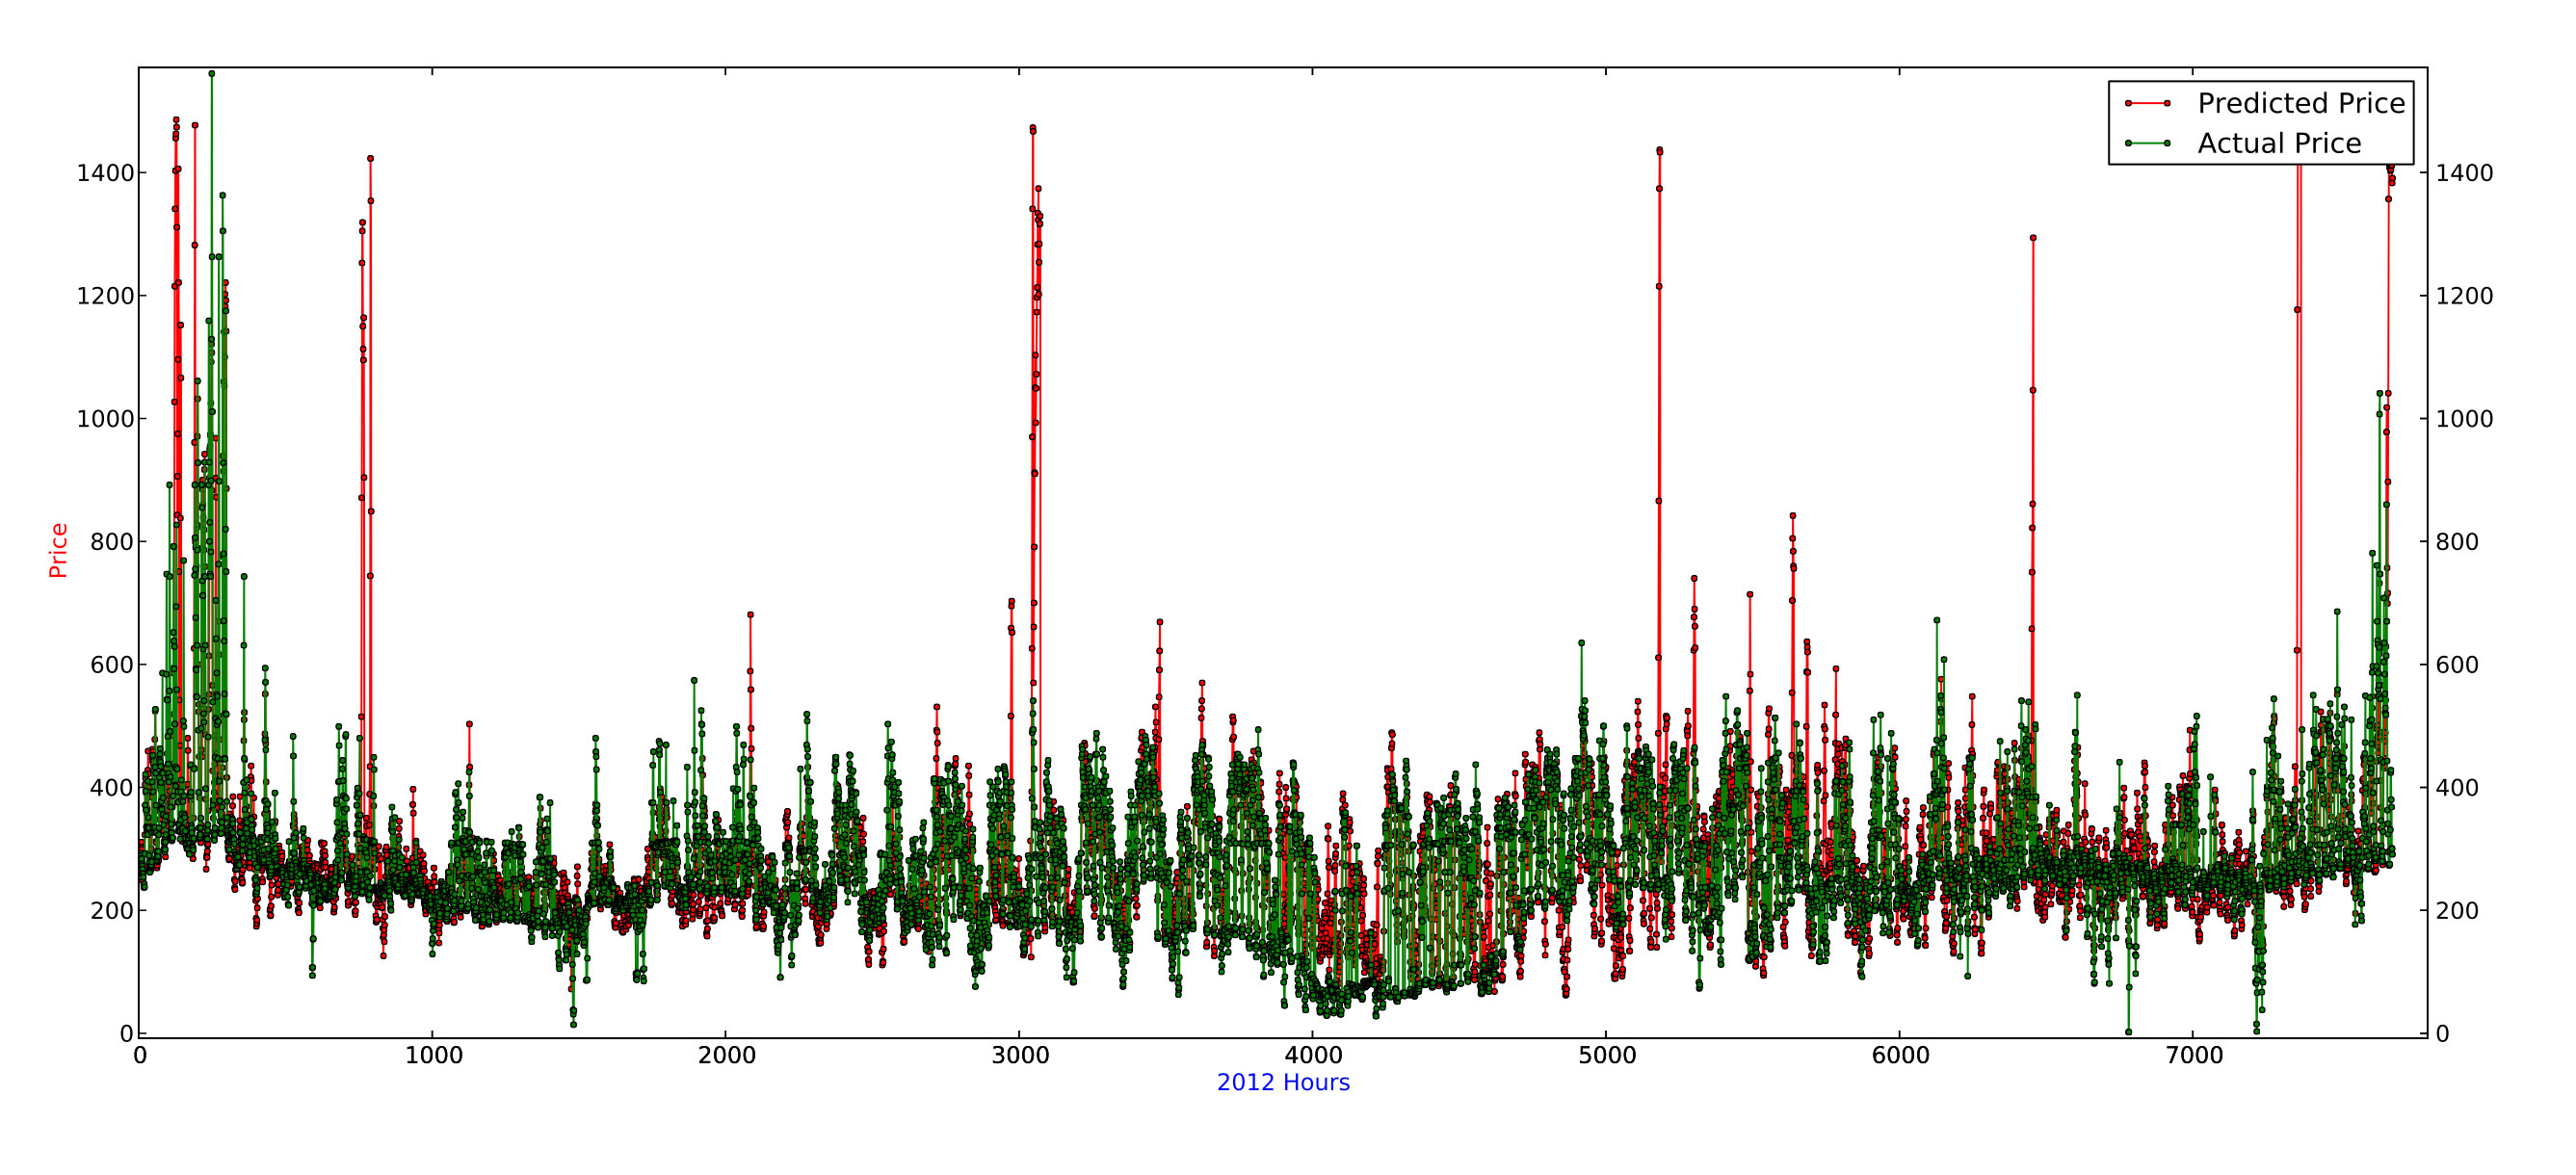
\includegraphics[width=0.85\linewidth,natwidth=898,natheight=587]{billeder/PriceExperimentalAnalysis/NoTrimming.jpg}
\caption{The \#1 forecast with no trimming of the dataset}
\label{fig:NoTrim}
\end{figure}

\begin{figure}[H]
\centering
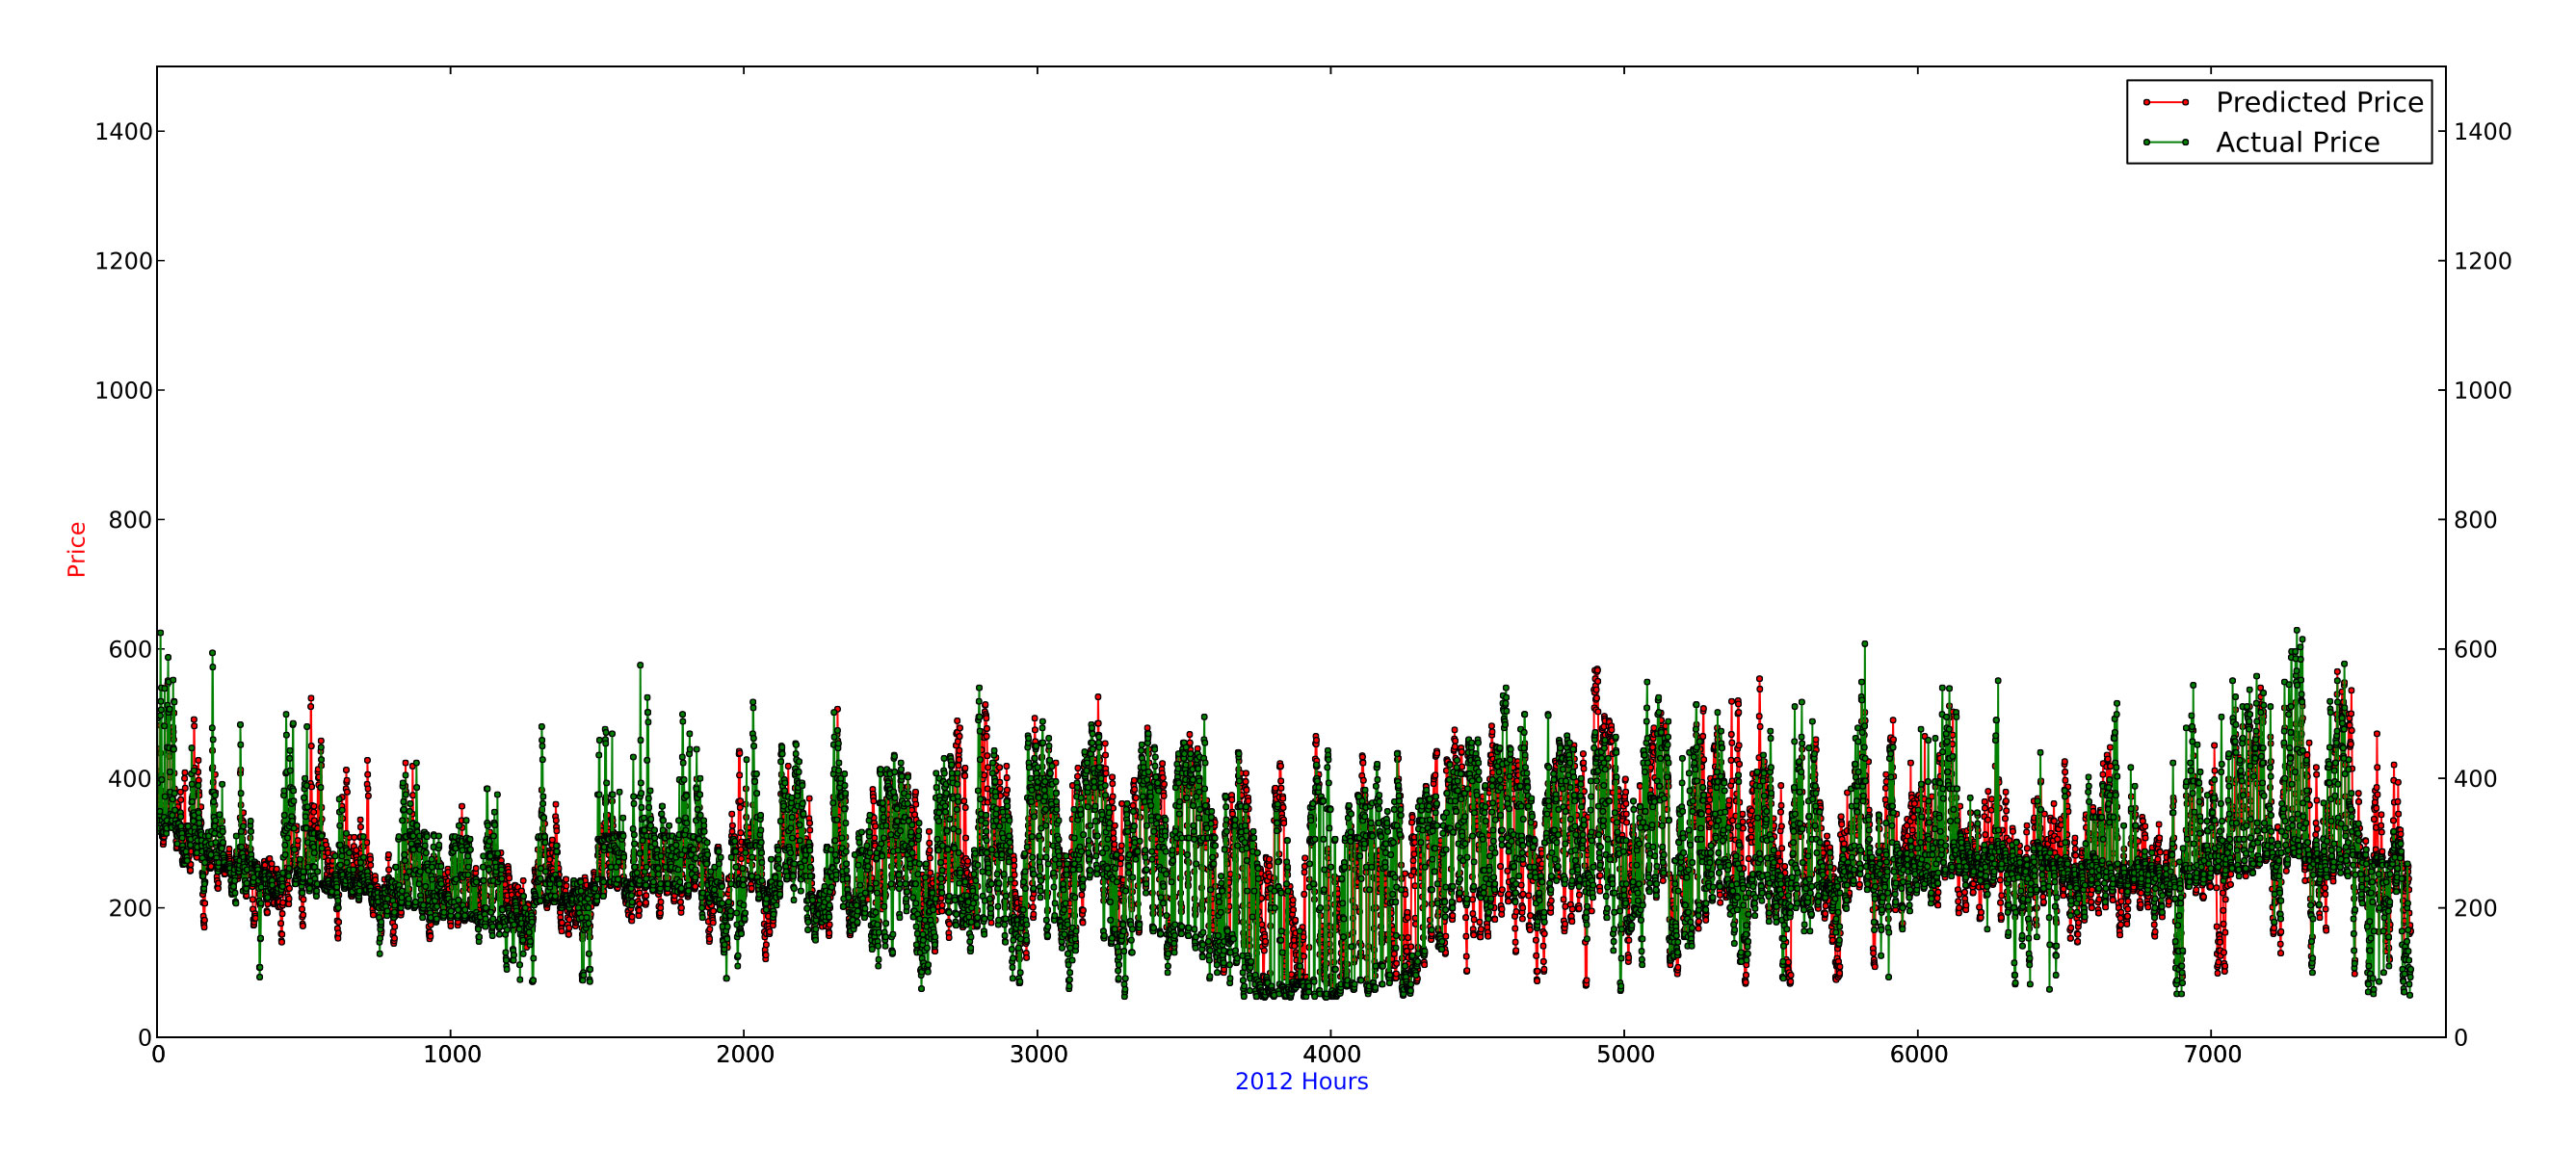
\includegraphics[width=0.85\linewidth,natwidth=898,natheight=587]{billeder/PriceExperimentalAnalysis/1PTrim.jpg}
\caption{The \#1 forecast with 1\% trimming in both ends of the dataset}
\label{fig:1PTrim}
\end{figure}

\begin{table}[H]
\centering  % used for centering table
\resizebox{0.6\textwidth}{!}{
	\begin{tabular}{c c c c c c} % centered columns (7 columns)
	1PTrim & 2PTrim & 3PTrim & 4PTrim & 5PTrim & Number\\ [0.5ex] % inserts table 
	\hline                  % inserts single horizontal line
	47,21 & 42,90 & 44,48 & 42,46 & 41,79 & \#1 \\
	46,15 & 43,67 & 43,07 & 39,16 & 40,28 & \#2 \\
	47,14 & 45,10 & 43,38 & 40,50 & 39,41 & \#3 \\
	46,70 & 43,96 & 43,21 & 40,03 & 40,29 & \#4 \\
	45,96 & 43,25 & 45,51 & 40,74 & 40,42 & \#5 \\
	47,27 & 45,96 & 44,98 & 41,39 & 39,98 & \#6 \\
	45,93 & 44,66 & 43,39 & 41,02 & 40,40 & \#7 \\
	46,64 & 42,69 & 44,48 & 41,69 & 40,61 & \#8 \\
	45,98 & 44,51 & 43,71 & 40,74 & 41,08 & \#9 \\
	45,60 & 46,07 & 45,81 & 42,52 & 41,32 & \#10 \\
	\hline %inserts single line
	\end{tabular}
}
\caption{Trims} % title of Table
\label{table:Top10Trimming} % is used to refer this table in the text
\end{table}

363 entries gets removed per percent.

\subsubsection{Experiment 3: Statistical strategies}

\subsubsection{Experiment 4: Black box optimization}

